\documentclass[aps,pre,noshowpacs]{revtex4}
\usepackage{bm}
\usepackage{graphicx}
%\usepackage{showlabels}
%\usepackage{showkeys}

\begin{document}
\title{RG flow through decimation of undetected degrees of freedom}

\author{Serena Bradde and William Bialek}
\maketitle
We want to give a reason why a system can be described by an effective hamiltonian
disregarding the details of real physical interactions also in absence of locality.
Neural networks or gene interaction networks are complicated networks
with an intrinsic non local structure but their joint probability distribution
can be described in terms of effective hamiltonian with two body interaction terms.

There is indeed a certain region of parameters, close to critical point in which parameters
are relevant or irrelevant. In this respect we can disregard irrelevant operator and still
we have a good description of joint probability distribution. This means that 
the effective model and the real one appear to be equivalent given the experimental accuracy.

Using mean field models, the paradigm of non local systems, we try to give a justification of 
how to select the relevant degrees of freedom to build the joint distribution of a collection of spins
by decimation. This procedure allow us to asses the stability of the model after integrating over
certain degrees of freedom.


\section{Ising model}

Let us start with a system of $N$ interacting spins with coupling $J$ with a Boltzmann joint probability distribution. 
If we observe just a part of it, we can write their joint probability distribution as
\begin{equation}\label{fullprob}
\mathcal{P}(\{\sigma_i\}) = \frac{1}{Z} e^{ \frac{\beta J}{2} \sum_{i j}  \sigma_i \sigma_j}  \sum_{\tau_a} e^{ \frac{\beta J}{2}\left( \sum_{ia} \sigma_i \tau_a + \sum_{ab} \tau_a \tau_b\right) }
\end{equation}
where $i$ and $j$ run over over all the couples of observed nodes while $a$ and $b$ run over the hidden variables. 
Suppose that the total number is $N$ and the fraction of hidden nodes is $x=N_h/N$, we need to
integrate over the hidden variable obtaining the final joint distribution in which the interaction
are renormalized.

\subsection{Mean field solution}

One way of doing is to use the fact that in mean field model  the energy of each configuration is just a function of the
magnetisation, $m=1/N(\sum_i \sigma_i +\sum_a \tau_a)$ so that, 
\begin{equation}\label{fullprob}
\mathcal{P}(\{\sigma_i, \tau_a\}) =  \frac{1}{Z} e^{-\beta N e(m)} \delta\left(\frac{1}{N} \sum_i \sigma_i + \frac{1}{N}\sum_a\tau_a-m \right)
\end{equation}
where the energy reads $e(m)=-J m^2/2$. Now we want to perform a partial sum
over the hidden variables.
In order to perform the calculation we start splitting the total magnetisation in two parts 
%$$\begin{array}{lll} \mbox{Observed: } & i \in \mathcal{A}& |\mathcal{A}| =(1-x) N \\ \mbox{Hidden: } & a \in \overline\mathcal{A} & |\overline\mathcal{A}|=xN\end{array}\,.$$ 
\begin{equation}\label{mag}
m= \frac{1}{N} \sum_{i } \sigma_i + \frac{1}{N}\sum_{a } \tau_a = (1-x) m_o + x m_h
\end{equation}
where $m_o=1/(N (1-x)) \sum_{i }\sigma_i $ is the effective magnetisation of the part we observe and $m_h= 1/(Nx)\sum_{a} \tau_a $ is the hidden one.
If we now write the probability of the observed subsystem, this will be the marginalization over the unobserved variables
\begin{equation}\label{subsytempdf}
\mathcal{P}(\{ \sigma\}) = \sum_{\{\tau\}} P(\{\sigma,\tau\}).
\end{equation}
and given the equation (\ref{fullprob}), we obtain for the joint distribution that
\begin{equation}\label{probmarg}
P(\{\sigma\}) = \frac{1}{Z}e^{N  \frac{\beta J (1-x)^2 }{2} m_o^2} \int dm_h \; e^{N \left( \frac{\beta J x^2}{2} m_h^2 +  x (1-x) \beta J m_o m_h \right)}\sum_{\tau}  \delta\left(\frac{1}{N x}\sum_{a} \tau_a-m_h\right)
\end{equation}
where the $\delta$ is the delta function. We know how to perform the sum over the unobserved nodes $\tau=\pm1$ when their total magnetization $m_h$ is fixed. Let us introduce the entropy
\begin{equation}\label{entropy}
s(m)=-\frac{1-m}{2}\log\left(\frac{1-m}{2}\right)-\frac{1+m}{2}\log\left(\frac{1+m}{2}\right)=-\frac{1}{2}\log\left(1-m^2\right) - \frac{m}{2} \log\left(\frac{1+m}{1-m} \right)+ \log2
\end{equation}
So that equation (\ref{probmarg}) reduces to
\begin{equation}\label{probmarg2}
P(\{\sigma\}) =\frac{1}{Z}e^{N (1-x)  \frac{\beta J (1-x) }{2} m_o^2} \int dm_h  \;e^{-N x \beta f(m_h,m_o)}
\end{equation}
where the free energy
\begin{equation}\label{freeenergy}
f(m,m_o)=-\frac{J x}{2} m^2 -  \frac{s(m) }{\beta} - J (1-x) m_o m\,.
\end{equation}
The free energy is the one associated to a smaller system of $Nx$ spins in presence of an external magnetic fieldgiven by the
magnetization of the observed systems $h= J(1-x) m_o$. 
In the limit of large system the integral in (\ref{probmarg2}) can be evaluate with a saddle point approximation. 
We thus get that the marginalized joint probability reads
\begin{equation}\label{probmarginal}
P(\{\sigma\}) = \frac{1}{Z}e^{N (1-x) \left(\frac{ \beta J (1-x) }{2} m_o^2 - \beta \frac{x}{1-x} f(\hat{m}_h, m_o)\right)}\,. 
\end{equation}
Remembering that $$\frac{\partial s}{\partial m}= - \frac{1}{2} \log\left(\frac{1+m}{1-m}\right)=-\mbox{atanh}(m)$$
we obtain the usual equation for the magnetization that extremizes the free energy 
in presence of an external field depending on the magnetization $m_o$
\begin{equation} \label{saddlemagn}
\hat{m}_h=\tanh(\beta J x \hat{m}_h + \beta J (1-x) m_o)\,.
\end{equation}
Substituting the solution $\hat{m}_h$ and dropping the index $h$, into (\ref{freeenergy}) we get
\begin{eqnarray}\label{fenergy_mhat}
f(\hat{m},m_o)&=& -\frac{J x}{2 } \hat{m}^2 - \frac{ s(\hat{m})}{\beta} - J (1-x) m_o \hat{m} =\nonumber\\
&=&-\frac{J x}{2} \hat{m}^2 +  \frac{1}{\beta} \left(\frac{ \log(1-\hat{m}^2) }{2}+\hat{m}\, \mbox{atanh}(\hat{m})\right) - J (1-x)  m_o \hat{m} - \frac{\log 2}{\beta}=\nonumber\\
&=&\frac{J x}{2} \hat{m}^2 +  \frac{1}{2\beta } \log(1-\hat{m}^2)- \frac{\log 2}{\beta}
\end{eqnarray}
where we use the equation (\ref{saddlemagn}) such that $\mbox{atanh}(\hat{m})=\beta J x \hat{m}_h + \beta J (1-x) m_o$. 
Now what we need to do is to explicit the dependence of $\hat{m}$ with respect to $m_o$ and then expand order by
order the logarithm to obtain all the higher oder terms. Let us start expanding first the logarithm 
\begin{equation}\label{smallexp}
f(\hat{m},m_o) \approx \frac{\beta J x -1}{2\beta} \hat{m}^2 -\frac{1}{4\beta} \hat{m}^4 -\frac{1}{6\beta} \hat{m}^6 + \ldots
\end{equation}
So that the final probability distribution for the observed system reads
\begin{equation}
P(\{\sigma\}) = \frac{1}{Z}e^{N_o \left(\frac{ \beta J (1-x) }{2}m_o^2 - \frac{x(\beta J x -1)}{2 (1-x)} \hat{m}^2 +\frac{x}{4(1-x)} \hat{m}^4 +\frac{x}{6 (1-x)} \hat{m}^6 + \ldots\right)}
\end{equation}
The final energy for the partial observed system contains thus higher order terms not just the two body interactions
\begin{equation}\label{energy}
e(m_o) = -\frac{J (1-x) }{2} m_o^2 +\frac{x(\beta J x -1)}{2\beta (1-x)} \hat{m}^2 -\frac{x}{4\beta(1-x)} \hat{m}^4 -\frac{x}{6 \beta (1-x)} \hat{m}^6 + \ldots
 \end{equation}
where we have an implicit dependence on the saddle point value, $\hat{m}$, on the magnetization $m_o$. 

\subsubsection{Above the critical temperature}

Whenever $\beta<\beta_c$ the dependence of $\hat{m}$ with respect to $m_o$ is easy accessible.
We need just to expand the saddle point equation (\ref{saddlemagn}). We thus get that first order and
\begin{eqnarray}
\hat{m}= \beta J x \hat{m} + \beta J (1-x) m_o - \frac{(\beta J (1-x)m_o)^3}{3} \;\Rightarrow\; \hat{m}= \frac{\beta J (1-x)}{ 1-\beta J x} m_o + o(m_o^3)
\end{eqnarray}
Using the expansion for the energy given in equation (\ref{energy}), we get that 
\begin{equation}\label{energy}
e(m_o) = -\frac{J (1-x) }{2 (1-\beta J x)} m_o^2  + o(m_o^4)
 \end{equation}
Let us define the new energy function for $N_o$ interacting spins such that
\begin{equation} 
P(\{ \sigma\}) = \frac{1}{Z} e^{-\beta N_o e(m_o)}
\end{equation}
where the energy now reads $ e(m_o)=  J_1 m_o+\frac{J_2}{2} m_o^2+ \frac{J_3}{3} m_o^3  +\ldots$
Given (\ref{energy}), we can easily identified the renormalized parameters
$$J_2= \frac{J (1-x) }{ (1-\beta J x)}$$
At the critical temperature, $\beta_c J =1$, the two body interaction term is independent on $x$, $J_2/J=1$. This means
that the system is identical to its subparts and it is not renormalized when we perform the integration over the hidden variables. 
Whenever $\beta J<1$, $J_2$ decreases and vanishes when $x=1$. We show the behaviors in the left panel of Figure \ref{fig:aboveTc}. Considering higher order terms, we need to be careful in the expansion that we be performed later.
\begin{figure}
\includegraphics[width=.7\columnwidth,angle=0]{AboveTc.pdf}
%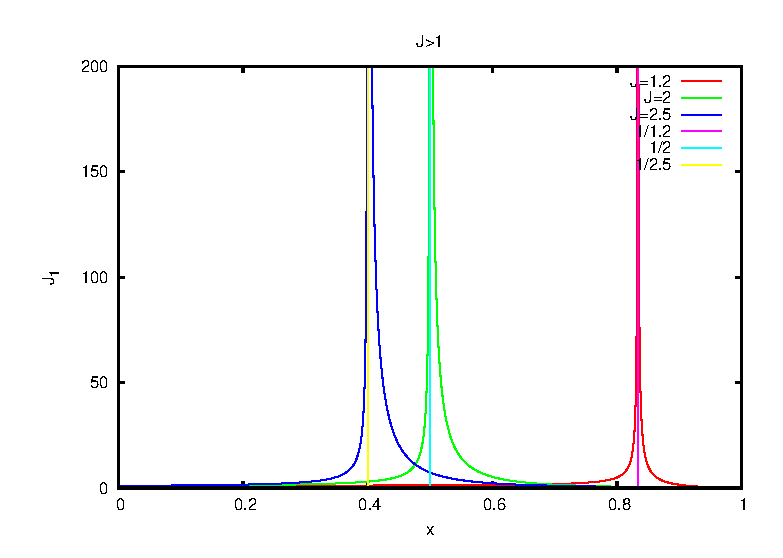
\includegraphics[width=.4\columnwidth,angle=0]{j_ordered.eps}
%\includegraphics[width=.6\columnwidth,angle=0]{jnew.eps}
\caption{We plot the effective interaction as function of the unobserved nodes $x$. On the left panel we show the behavior of 
the renormalized coupling $J_2/J$ for different values of $\beta J$. The closer to the critical point the less the hidden nodes affect
the interaction. While in the right panel we show the behavior of $-(1-x) J_4/J_2<1/3$. The 4-body interaction term is always smaller and negative with respect to the 2 body interaction term. The factor $1-x$ is added to compare dimensionless parameter $J_4$ with respect to the dimensionless parameter $J_2$.}
\label{fig:aboveTc}
\end{figure}


\subsubsection{Below the critical temperature}

The general analysis valid also below the critical temperature follows the lines of the previous one. 
First of all we need to expand the saddle point solution (\ref{saddlemagn}) when a non vanishing zero solution appears. 
In particular we search for the coefficient 
$\hat{m}=\overline{m} + a_1 m_o +a_2 m_o^2 +a_3 m_o^3 + \ldots $

Those can be identified through order by order expansion of (\ref{saddlemagn}) and we get that
\begin{eqnarray}
\overline{m}&=&\tanh( \beta J x \overline{m})\nonumber\\
a_1&=&\frac{\beta  J \left( \overline{m}^2-1\right) (x-1)}{\beta  J x\left( \overline{m}^2-1\right) +1}\nonumber \\
a_2 &=& \frac{\beta^2J^2 \overline{m} \left(\overline{m}^2-1\right) (x-1)^2}{\left(\beta J x \left(\overline{m}^2-1\right) +1\right)^3}\nonumber\\
a_3 &=&-\frac{\beta ^3 J^3 \left(\overline{m}^2-1\right) (x-1)^3 \left(3 \beta  J x \overline{m}^4 -\overline{m}^2 (2 \beta  J x+3)-\beta  J x+1\right)}{3 \left(\beta  J x\left(\overline{m}^2-1\right) +1\right)^5}\nonumber\\
a_4 &=&\frac{\beta ^4 J^4 \overline{m} \left(\overline{m}^2-1\right) (x-1)^4 \left(3 \beta ^2 J^2 x^2 \overline{m}^6 +\overline{m}^2 \left(-3 \beta ^2 J^2 x^2+10 \beta  J x+3\right)+3 \beta ^2 J^2 x^2-3 \beta  J \overline{m}^4 x (\beta  J x+3)-\beta  J x-2\right)}{3 \left(\beta  J x\left(\overline{m}^2-1\right) +1\right)^7} \nonumber\\
%a_5&=&-\frac{\beta ^5 J^5 \left(\overline{m}^2-1\right) (x-1)^5 \left(15 \beta ^3 J^3 \overline{m}^{10} x^3-15 \beta ^2 J^2 \overline{m}^8 x^2 (\beta  J x+6)+6 \beta  J \overline{m}^6 x \left(-7 \beta ^2 J^2 x^2+25 \beta  J x+15\right)+\overline{m}^4 \left(66 \beta ^3 J^3 x^3-26 \beta ^2 J^2 x^2-135 \beta  J x-15\right)+\overline{m}^2 \left(-21 \beta ^3 J^3 x^3-38 \beta ^2 J^2 x^2+44 \beta  J x+15\right)-(\beta  J x-1)^2 (3 \beta  J x+2)\right)}{15 \left(\beta  J x\left(\overline{m}^2-1\right) +1\right)^9}\nonumber
\end{eqnarray}
After that we can identify all the interaction terms order by order. This is due to the fact that once you have a general energy
density function $e(m_o)=J_1 m_o + J_2 m_o^2/2 +\ldots$, we get that given the usual free energy definition
\begin{equation}
f(m_o)=e(m_o)- s(m_o)/\beta
\end{equation}
we get a self consistent equation of the following type 
\begin{equation}\label{jkdef}
m_o=\tanh( \beta J_1 + \beta J_2 m_o + \beta J_3 m_o^3 + \beta J_4 m_o^4 +\ldots)
\end{equation}
where we can identify all the $J_k$ with the term in the expansion.
So let us obtain the self consistent equation for $m_o$. We should derive the free energy with respect to $m_o$, $\partial_{m_o} f(\hat{m},m_o)=0$.  In particular in our case since $\hat{m}$ is a function of $m_o$ itself and knowing that $\partial_{m_o} \hat{m} = (1-\hat{m}^2) \beta J (1-x)$, we get using the free energy (\ref{fenergy_mhat}) that
\begin{eqnarray}
&&- J (1-x)^2 m_o - J x^2 \hat{m}\frac{ \partial \hat{m}}{\partial m_o} - J x (1-x) \hat{m} - J x (1-x) m_o \frac{ \partial \hat{m}}{\partial m_o} - \frac{x}{\beta} \mbox{atanh}(\hat{m}) \frac{ \partial \hat{m}}{\partial m_o} + \frac{1-x}{\beta} \mbox{atanh}(m_o)=0\nonumber\\
 &&m_o= \tanh\left(\beta J (1-x) m_o + \beta J x \hat{m}\right) 
\end{eqnarray}
where we use the fact that $\mbox{atanh}(\hat{m})=\beta J x \hat{m} + \beta J (1-x) m_o$ and those cancel all the terms dependent on $\partial_{m_o} \hat{m}$. 
Since $\hat{m}=\overline{m} + a_1 m_o + a_2 m_o^2 + \ldots $, we get that the self consistent equation reads
$$ m_o=\tanh\left(\beta J x \overline{m}+ \beta (J (1-x) +J x a_1 ) m_o + \beta J x a_2 m_o^2 + \beta J x a_3 m_o^3 + \ldots \right)\,.$$ As showed by equation (\ref{jkdef}), we are thus able to identify the new coupling $J_k$ in terms of the parameters $a_i$'s
\begin{eqnarray}\label{renJ1hT}
J_1&=& J x \overline{m} \nonumber\\
J_2&=&  J(1-x) + Jx a_1\nonumber\\
J_3&=&Jx a_2\nonumber\\
J_4&=& J xa_3\nonumber\\
J_5&=&Jx a_4\nonumber\\
J_6&=&Jx a_5\nonumber\\
\end{eqnarray}


Whenever $\beta J <1$, there will be only one solution around zero $\overline{m}=0$ namely the hidden system is disordered, so $\hat{m}$ is an odd function of $m_o$ such that the things simplify
\begin{eqnarray}
a_1&=& \frac{\beta  J (1-x)}{1-\beta  J x} \;\Rightarrow \; J_2=J(1-x) + Jx a_1=\frac{J(1-x)}{1-\beta J x}\nonumber \\
a_2 &=& 0 \nonumber\\
a_3 &=& -\frac{\beta ^3 J^3 (1-x)^3}{3 (1-\beta  J x)^4} \;\Rightarrow \; J_4= Jx a_3=-\frac{\beta^3 J^4 (1-x)^3 x}{3(1-\beta J x)^4}\nonumber\\
a_4 &=& 0\nonumber\\
%a_5&=&\frac{\beta ^5 J^5 (x-1)^5 (3 \beta  J x+2)}{15 (\beta  J x-1)^7}
\end{eqnarray}
recovering the result above the critical temperature and obtaining also higher order terms.

Below critical temperature $\beta J>1$ we need to distinguish two cases: 
\begin{itemize}
\item above the hidden system critical temperature $\beta J x<1$. This means that $x<1/\beta J$ that is in the range below the unity  and also $(1-\beta J x )>0$. In this regime, $\overline{m}=0$ so that the parity of the free energy is recovered $J_1=J_3=J_5=0$.
The system is thus not stable and diverge to infity at a critical value $x_c=1/\beta J$. This is due to the fact that the system developed a long range correlation so the renormalization procedure
flows to strong coupling. The interactions are as above the critical temperature
\begin{eqnarray}
J_2= \frac{J (1-x)}{1-\beta  J x} \qquad J_4=-\frac{\beta ^3 J^4 x (1-x)^3 }{3 (1-\beta  J x)^4} \qquad J_6 = \frac{\beta ^5 J^6 (x-1)^5 x (3 \beta  J x+2)}{15 (\beta  J x-1)^7}
\end{eqnarray}
In this regime the denominator of $J_2$ diverge at the critical value $x_c=1/\beta J$. The system exhibits a strong coupling behavior meaning that the variables get strongly coupled. 
\item below the hidden system critical temperature $\beta J x >1$. We should consider the onset of a non null magnetization $\overline{m}$. This makes calculation more complicated but we can still plot the result for $J_2/J$ and $J_4$ to show their 
behavior flows to strong coupling limit as you see in  Figure \ref{fig:belowTc}
\end{itemize}
\begin{figure}
%\includegraphics[width=.7\columnwidth,angle=0]{}
%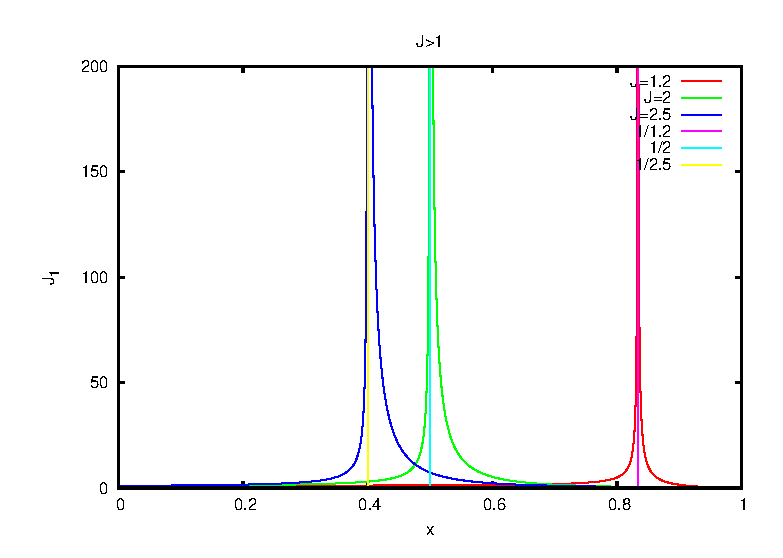
\includegraphics[width=.4\columnwidth,angle=0]{j_ordered.eps}
%\includegraphics[width=.6\columnwidth,angle=0]{jnew.eps}
\caption{We plot the effective interaction as function of the unobserved nodes $x$. On the left panel we show the behavior of 
the renormalized coupling $J_2/J$ for different values of $\beta J$ below the critical temperature $\beta J >1$.}
\label{fig:belowTc}
\end{figure}


\subsection{Dimension and relevant operators}

Let us discuss their dimensions as function of the renormalization parameter $b=1/(1-x)$. We know that above the critical temperature $\sigma_o=1/(b^{\omega}) \sum_{i=1}^{b} \sigma_i $. Since we have the gaussian fix point  where every variable is independent with null mean value and fixed variance $\Delta$, we have that $$\langle \sigma_o^2\rangle = b^{1-2 \omega} \langle \sigma^2\rangle $$ So that the dimension of the magnetization is $\omega=1/2$. In this regime when integrating over $b=1/(1-x)$ variables we get that $m_o \to m_o \sqrt{b}$. After rescaling $N \to N /b$, so in order to keep the energy invariant $\mathcal{E}_o \to \mathcal{E}_o$ we have that
$$J_2 \to J_2  \qquad J_4 \to  J_4 b \qquad J_6 \to J_6 b^2\,.$$
We thus need to define the renormalized running coupling constant removing the dependence of the dimension such that the adimensional coupling constant $J^a_2=J_2$ while $J^a_4=J_4 / b=J_4 (1-x) $ and $J^a_6=J_6 /b^2=J_6(1-x)^2$ that will be the relevant parameters plotted in figures \ref{fig:aboveTc} and.... 


We can define the beta function for this quantities that is the log derivative in terms of the running constants. Concerning the two body interaction beta function
\begin{equation}
-\beta_2(J^a_2) = (1-x) \frac{\partial \log J^a_2}{\partial (1-x)} =-(1-x) \frac{\partial \log J^a_2}{\partial x} = \frac{\beta J -1}{\beta J x -1} = 1-\beta J^a_2 =
\end{equation}
so we get a fixed point $\beta J^a_2=1$. In the same way we get the four body interaction term
\begin{equation}
-\beta_4(J^a_2, J^a_4) = (1-x) \frac{\partial \log J^a_4}{\partial (1-x)} =-(1-x) \frac{\partial \log J^a_4}{\partial x} = \frac{\beta  J x^2+x (3 \beta  J-5)+1}{x (\beta  J x-1)}
\end{equation}
In terms of the adimensional running coupling constants we have that 
\begin{equation}
-\beta_4(J^a_2, J^a_4)  =   2 + 3(1-\beta J^a_2) - \beta J^a_2\left(1-\frac{(\beta J^a_2)^3}{3\beta J^a_4} \right)
\end{equation}
At the fixed point $\beta J^a_2=1$ we get that the $J^a_4$ has a fixed point at $-1/3$. 
Instead for the last coupling constant $J^a_6$ 
\begin{equation}
\beta_6(J^a_2, J^a_4,J^a_6) = 4+ (1-\beta J'_2) \left(5 + \frac{6}{5} \frac{(\beta J^a_4)^2}{\beta J^a_6 (\beta J^a_2)^2}\right)- 2\beta J^a_2 \left( 1+ \frac{1}{15} \frac{(\beta J^a_2)^5}{ \beta J^a_6} - \frac{3}{5}  \frac{(\beta J^a_2)^2 \beta J^a_4}{\beta J^a_6}\right) 
\end{equation}




-What about spin glass in mean field?
-What about dimensional system with known RG fixed point?
\begin{figure}[h]
%\includegraphics[width=.5\columnwidth]{phasediagram.pdf}
\caption{In figure we sketch the phase diagram of the system as a function of the parameter $J$. If $J=1$ the system is not renormalized by the decimation procedure. Interestingly, when $J<1$ the system flows to the high temperature fixed point while
for $J>1$ we get that the system is going to the strong coupling regime. It is important to emphasize that although the two subsystems may appear to have lower critical temperatures, they know to be in the ordered phase and the effective coupling gets stronger and stronger increasing the fraction of unobserved nodes $x$.}
\end{figure} 
\end{document}